
% To generate the image first run:
% $> pdflatex mode1.tex
% Then run:
% $> convert -density 300 mode1.pdf -quality 90 mode1.png
% To include in a Markdown cell of a netbook then use something like:
% <img src="images/mode1.png" alt="Drawing" style="width: 200px;"/>

\documentclass{standalone}

\usepackage{tikz}
\usetikzlibrary{patterns}

\begin{document}

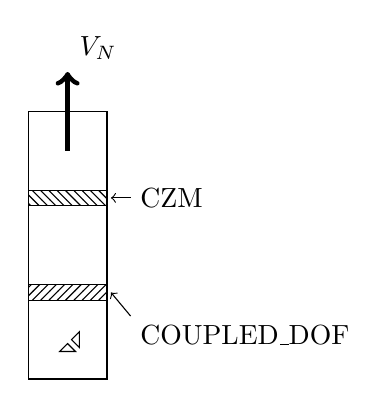
\begin{tikzpicture}

  % first block
  \draw (0., 0.) rectangle (1. , 1.)  ;

  % fixed BC on first block
  \draw (0.5 , 0.45) -- (0.4 , 0.35) -- (0.6 , 0.35) -- cycle ;
  \draw (0.55, 0.5 ) -- (0.65, 0.4 ) -- (0.65, 0.6 ) -- cycle ;

  % coupled dof zone
  \draw [pattern=north east lines] (0. , 1.) rectangle (1., 1.2) ;
  \draw [<-] (1.05, 1.1) -- (1.3, 0.8) node[below right] {COUPLED\_DOF} ;

  % second block
  \draw (0., 1.2) rectangle (1., 2.2) ;

  % CZM
  \draw [pattern=north west lines] (0. , 2.2) rectangle (1., 2.4) ;
  \draw [<-] (1.05, 2.3) -- (1.3, 2.3) node[right] {CZM} ;

  % third block
  \draw (0., 2.4) rectangle (1.  , 3.4) ;

  % force BC on third block
  \draw[line width=2pt, ->]  (0.5  , 2.9) -- (0.5  , 3.9) node[above right] {$V_N$};

\end{tikzpicture}

\end{document}
